%! TeX program = lualatex
\documentclass[../main.tex]{subfiles}
\begin{document}
\begin{lesson}{Derivatives and the shape of a graph}

  \begin{center}
    \begin{tikzpicture}
      \begin{axis}[enlargelimits, width=2in, smooth, samples=100, xtick=\empty, ytick=\empty, axis lines=box, gray!40, xlabel={}, ylabel={}]
        \addplot[black, domain=-0.9:0] {sqrt(1-x^2)};
      \end{axis}
    \end{tikzpicture}
    \quad
    \begin{tikzpicture}
      \begin{axis}[enlargelimits, width=2in, smooth, samples=100, xtick=\empty, ytick=\empty, axis lines=box, gray!40, xlabel={}, ylabel={}]
        \addplot[black, domain=0:0.9] {-sqrt(1-x^2)+1};
      \end{axis}
    \end{tikzpicture}
    \quad
    \begin{tikzpicture}
      \begin{axis}[enlargelimits, width=2in, smooth, samples=100, xtick=\empty, ytick=\empty, axis lines=box, gray!40, xlabel={}, ylabel={}]
        \addplot[black, domain=0:0.9] {sqrt(1-x^2)};
      \end{axis}
    \end{tikzpicture}
    \quad
    \begin{tikzpicture}
      \begin{axis}[enlargelimits, width=2in, smooth, samples=100, xtick=\empty, ytick=\empty, axis lines=box, gray!40, xlabel={}, ylabel={}]
        \addplot[black, domain=-0.9:0] {-sqrt(1-x^2)+1};
      \end{axis}
    \end{tikzpicture}
  \end{center}

  \begin{mdframed}[style=simple-compact]
    \begin{enumerate}[label=(\alph*)]
      \item If \underline{\hspace{1.5in}} for every \(x\) in \(I\), then \(f(x)\) is increasing on \(I\).
      \item If \underline{\hspace{1.5in}} for every \(x\) in \(I\), then \(f(x)\) is decreasing on \(I\).
    \end{enumerate}
  \end{mdframed}

  \faStar{} If \(f'(c) = 0\) for some constant \(c\), then \(f(x)\) is \underline{\hspace{3.5in}}.

  \begin{example}
    Consider the graph of \(f'(x)\) below. On the horizontal axis, label the interval on which \(f(x)\) is increasing. 

    \begin{center}
      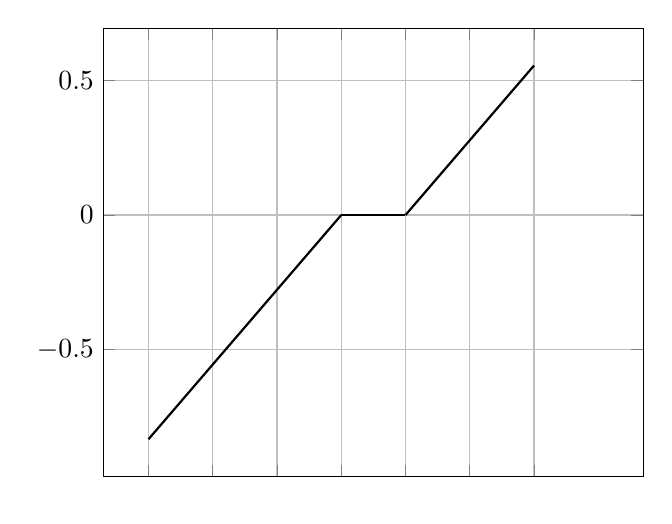
\begin{tikzpicture}
        \begin{axis}[
          axis lines = box,
          axis equal image=false,
          enlargelimits=true,
          xmin=-3*pi/2, xmax=2*pi,
          xtick={-3*pi/2, -pi, -pi/2, 0, pi/2, pi, 3*pi/2},
          xticklabels={},
          grid=major,
          ]
          \addplot[thick, black, domain=-3*pi/2:0] {sin(x) + x/2/pi};
          \addplot[thick, black, domain=0:pi/2] {0};
          \addplot[thick, black, domain=pi/2:3*pi/2] {sin(x-pi/2) + (x-pi/2)/2/pi};
          \node[above left] at (axis cs:1,1) {\footnotesize \(f'(x)\)};
        \end{axis}
      \end{tikzpicture}
    \end{center}
  \end{example}

  We learned that critical points are candidates for local extrema. Let's learn two tests to determine if a critical point is a local extrema or not.

  The idea: If \(f(x)\) has a local extrema at \(c\), then \((c,f(c))\) must be the ``peak or valley of a mountain.''  We simply look left and right.
  \begin{center}
    \includegraphics[scale=0.8]{../standalones/build/plot_increasing_decreasing}
    \hfill
    \includegraphics[scale=0.8]{../standalones/build/plot_increasing_decreasing_only_derivative}
    \hfill
    \includegraphics[scale=0.8]{../standalones/build/plot_increasing_decreasing_with_derivative}

    \url{https://www.geogebra.org/calculator/atcbwgvm}
  \end{center}
  \clearpage

  \begin{mdframed}[style=withref-compact]
    Suppose that \(f\) is a continuous function over an interval \(I\) containing a critical number \(c\). 

    If \(f\) is differentiable over \(I\), except possibly at \(c\), then \(f(c)\) satisfies one of the following descriptions:
    \begin{enumerate}
      \item If \(f'\) \emph{changes} sign from positive when \(x < c\) to negative when \(x > c\), then \(f\) has a \underline{\hspace{2in}} at \(c\).
      \item If \(f'\) \emph{changes} sign from negative when \(x < c\) to positive when \(x > c\), then \(f\) has a \underline{\hspace{2in}} at \(c\).
      \item If \(f'\) has the same sign for \(x < c\) and \(x > c\), then \(f(c)\) has neither a local maximum nor a local minimum of \(f\).
    \end{enumerate}

    \textbook{Theorem~4.9 First Derivative Test on page 392}
  \end{mdframed}

  \begin{example}[Textbook Example~4.18] \label{ex:first-derivative}
    Use the first derivative test to find the location of all local extrema for \(f(x) = 5x^{1/3} - x^{5/3}\). Graph: \url{https://www.geogebra.org/calculator/nzwzefct}

    \blanklines{25}
  \end{example}
  \clearpage

  We can dig up more information about a function by considering concavity.
  \begin{mdframed}[style=withref-compact]
    Let \(f\) be a differentiable function over an \emph{open} interval \(I\).
    \begin{itemize}
      \item If \(f'\) is \underline{\hspace{1in}} over \(I\), then we say \(f\) is \hlmain{concave up}.
      \item If \(f'\) is \underline{\hspace{1in}} over \(I\), then we say \(f\) is \hlmain{concave down}.
      \item If \(f\) is continuous at \(c\) and changes concavity at \(c\), then \((a,f(a))\) is an \hlmain{inflection point}. 
    \end{itemize}

    \textbook{Definition on page 395 and 397}
  \end{mdframed}

  \begin{center}
    \includegraphics[scale=0.8]{../standalones/build/plot_concavity}
    \hfill
    \includegraphics[scale=0.8]{../standalones/build/plot_concavity_only_derivative}
    \hfill
    \includegraphics[scale=0.8]{../standalones/build/plot_concavity_with_derivative}

    \url{https://www.geogebra.org/calculator/atcbwgvm}
  \end{center}

  \begin{mdframed}[style=withref-compact]
    Let \(f\) be a function whose second derivative exists over an interval \(I\).
    \begin{itemize}
      \item If \underline{\hspace{1in}} on an interval \(I\), then the graph of \(f\) is \hlmain{concave up} on \(I\).
      \item If \underline{\hspace{1in}} on an interval \(I\), then the graph of \(f\) is \hlmain{concave down} on \(I\).
    \end{itemize}

    \textbook{Theorem 4.0 Test for Concavity on page 396}
  \end{mdframed}

  \begin{example} \label{ex:concavity}
    Let \(f = x^{4} - 4x^{3}\). Find all intervals on which \(f\) is concave up and all intervals on which \(f\) is concave down. List all inflection points of \(f\).

    \blanklines{18}
  \end{example}

  \clearpage

  When a function is twice differentiable, the Second Derivative Test \hlmain{could be a faster method} for finding local extrema.

  \begin{mdframed}[style=withref-compact]
    Suppose \(f'(c) = 0\) and \(f''\) is continuous near \(c\).
    \begin{itemize}
      \item If \(f''(c) > 0\) (meaning \(f\) is \underline{\phantom{concave down}} near \(c\)), then \(f\) has a \underline{\hspace{1in}}.
      \item If \(f''(c) < 0\) (meaning \(f\) is \underline{\phantom{concave down}} near \(c\)), then \(f\) has a \underline{\hspace{1in}}.
      \item[\faExclamationTriangle{}] If \(f''(c) = 0\) or \(f''(c)\) does not exists, then the Second Derivative Test is \hlwarn{inconclusive} meaning that we need to \hlsupp{explore other methods} to determine if \(f\) has a local extrema at \(c\).
    \end{itemize}

    \textbook{Theorem~4.11 Second Derivative Test on page 400}
  \end{mdframed}

  \begin{example}
    Use the Second Derivative Test to find all local extrema for \(f(x) = x^{4} - 4x^{3}\) from Example~\ref{ex:concavity}.
    \blanklines{35}
  \end{example}
  \vfill
\end{lesson}
\end{document}
